\documentclass[aspectratio=169,10pt,professionalfonts]{beamer}

\usepackage{xeCJK}
\usepackage{fontspec}
\usepackage{amsmath}
\usepackage{amssymb}
\usepackage{booktabs}
\usepackage{multirow}
\usepackage{array}
\usepackage{graphicx}
\usepackage{xcolor}
\usepackage{pgfplots}
\usepackage{adjustbox}
\usepackage{hyperref}

\pgfplotsset{compat=1.18}
\hypersetup{hidelinks}

\setmainfont{TeX Gyre Termes}
\setsansfont{TeX Gyre Heros}
\setmonofont{Latin Modern Mono}
\setCJKmainfont{Noto Serif CJK SC}
\setCJKsansfont{Noto Sans CJK SC}
\setCJKmonofont{Noto Sans Mono CJK SC}

\makeatletter
\def\input@path{{theme/}}
\makeatother
\usetheme{XDU}

\title{基于 XDU 模板的 Beamer 演示文稿}
\subtitle{本科答辩 / 课程汇报 / 学术报告}
\author{张三}
\institute{电子工程学院}
\advisor{李四教授}
\date{2026 年 5 月}

\begin{document}

\makexdutitle
\makexduoutline

\section{模板概览}

\begin{frame}{模板定位}{What This Template Provides}
  \vspace{0.10cm}
  \begin{columns}[T,totalwidth=\textwidth,onlytextwidth]
    \begin{column}{0.48\textwidth}
      \cardbox{0.62\textheight}{核心能力}{%
        \begin{itemize}\setlength\itemsep{0.95em}
          \item 统一封面、目录、章节分隔页
          \item 内容页自动带页眉、页码与学校视觉元素
          \item 支持\hl{中英文混排}与图表展示
          \item 适合答辩、汇报、课程展示等场景
        \end{itemize}}
    \end{column}
    \begin{column}{0.48\textwidth}
      \cardbox{0.62\textheight}{使用方式}{%
        \begin{itemize}\setlength\itemsep{0.95em}
          \item 修改标题、作者、导师、单位、日期
          \item 按章节组织内容
          \item 复用 \texttt{\textbackslash cardbox}、\texttt{\textbackslash hl}、\texttt{\textbackslash numbadge}
          \item 运行 \texttt{make pdf} 直接生成 PDF
        \end{itemize}}
    \end{column}
  \end{columns}
\end{frame}

\begin{frame}{内容组织建议}{Recommended Structure}
  \vspace{0.10cm}
  \begin{columns}[T,totalwidth=\textwidth,onlytextwidth]
    \begin{column}{0.31\textwidth}
      \cardbox{0.58\textheight}{\numbadge{01} 背景}{%
        \begin{itemize}\setlength\itemsep{0.60em}
          \item 研究背景
          \item 问题定义
          \item 目标与意义
        \end{itemize}}
    \end{column}
    \begin{column}{0.31\textwidth}
      \cardbox{0.58\textheight}{\numbadge{02} 方法}{%
        \begin{itemize}\setlength\itemsep{0.60em}
          \item 总体架构
          \item 关键设计
          \item 方案优势
        \end{itemize}}
    \end{column}
    \begin{column}{0.31\textwidth}
      \cardbox{0.58\textheight}{\numbadge{03} 结果}{%
        \begin{itemize}\setlength\itemsep{0.60em}
          \item 实验设置
          \item 结果分析
          \item 总结与展望
        \end{itemize}}
    \end{column}
  \end{columns}
\end{frame}

\section{示例页面}

\begin{frame}{图文混排示例}{Example Slide}
  \vspace{0.10cm}
  \begin{columns}[T,totalwidth=\textwidth,onlytextwidth]
    \begin{column}{0.56\textwidth}
      \begin{minipage}[t][0.64\textheight][c]{\linewidth}
        \centering
        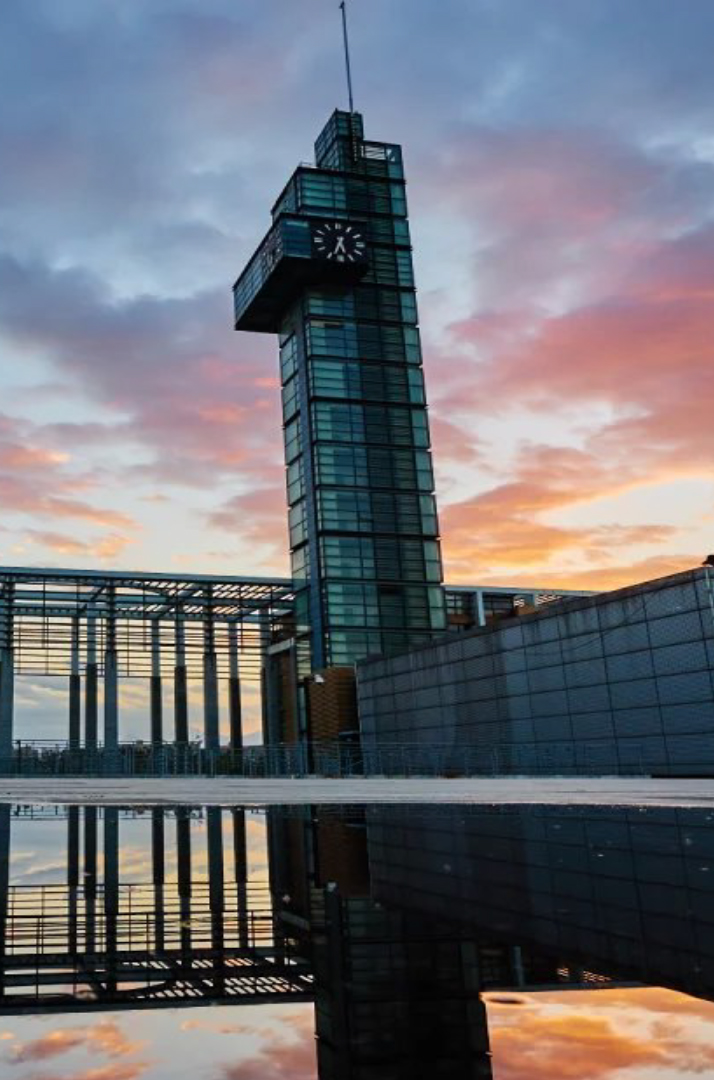
\includegraphics[width=\linewidth,height=0.60\textheight,keepaspectratio]{assets/section_bg.jpg}
      \end{minipage}
    \end{column}
    \begin{column}{0.40\textwidth}
      \cardbox{0.64\textheight}{展示建议}{%
        \begin{itemize}\setlength\itemsep{0.85em}
          \item 左图右文是答辩中最稳妥的结构
          \item 右侧只保留\hl{3 到 4 个}核心结论
          \item 每页尽量只传递一个主要信息
          \item 图表标题建议直接写成结论句
        \end{itemize}}
    \end{column}
  \end{columns}
\end{frame}

\begin{frame}{表格示例}{Table Example}
  \vspace{0.18cm}
  {\small
  \renewcommand{\arraystretch}{1.35}
  \begin{tabular}{@{}p{0.22\textwidth}p{0.24\textwidth}p{0.42\textwidth}@{}}
    \toprule
    \bfseries 页面类型 & \bfseries 适用场景 & \bfseries 建议内容 \\
    \midrule
    封面页 & 首屏展示 & 题目、汇报人、导师、单位、日期 \\
    章节页 & 大纲切换 & 章节编号、章节标题、视觉分隔 \\
    内容页 & 主体论述 & 图表、方法、结果、关键结论 \\
    致谢页 & 结束收束 & 感谢聆听、答辩结束提示 \\
    \bottomrule
  \end{tabular}}
  \vspace{0.35cm}
  \begin{center}
    \color{xdured}\bfseries\small 模板目标不是替你写内容，而是稳定地承载内容
  \end{center}
\end{frame}

\section{结束页}

\begin{frame}{总结}{Summary}
  \vspace{0.10cm}
  \begin{columns}[T,totalwidth=\textwidth,onlytextwidth]
    \begin{column}{0.48\textwidth}
      \cardbox{0.62\textheight}{模板收益}{%
        \begin{itemize}\setlength\itemsep{1.00em}
          \item 提供统一的 XDU 幻灯片视觉风格
          \item 降低每次从零搭建答辩稿的成本
          \item 保持版式规范、易改、可复用
        \end{itemize}}
    \end{column}
    \begin{column}{0.48\textwidth}
      \cardbox{0.62\textheight}{后续可扩展方向}{%
        \begin{itemize}\setlength\itemsep{1.00em}
          \item 增加英文版封面宏
          \item 增加参考文献页与附录页样式
          \item 增加浅色 / 深色双主题切换
        \end{itemize}}
    \end{column}
  \end{columns}
\end{frame}

\thankyouframe

\end{document}
